\section{Motivation}
{Wenn heutzutage die Spezifikation eines Projektes in Englisch formuliert wird, ist diese Spezifikation von Anfang an mehrdeutig, behauptet Jeannette Wing, Coperate Vice President von Microsoft Research. Des Weiteren sagt sie, dass jede natürliche Sprache mehrdeutig ist. Hingegen in formalen Spezifikationen, wird basierend auf Mathematik präzise erklärt, was genau ein Programm machen soll.}\cite{WING01:FV}
\\
\\
Diese Seminararbeit soll einen tieferen Einblick in den Themenbereich der Programmcodeverifikation schaffen. Dabei wird sowohl auf die Grundlagen als auch technisch-detaillierte Beispiele eingegangen. Als technisches Mittel wird hierfür der Proof-Assistent Coq verwendet.


\section{Warum ist Formale Verifikation interessant?}
Es existieren unzählige Beispiele für die Relevanz von Formaler Verifikation. Zum Beispiel jeder Computer besteht aus vielen elektronischen Hardwareteilen wie Prozessoren, Grafikkarte et cetera. Um diesen nutzen zu können, wird eine Hardware Description Language (HDL) eingesetzt. Diese beschreibt sowohl die Struktur als auch das Verhalte des elektronischen Bauteils.\\
Eine Firma X verkauft nun einen Computer mit einer fehlerhaften HDL-Software. Je nach Ausmaß des Bugs, kann dies gravierende Folgen nach sich ziehen.\\
\\
Heutzutage gehen viele Computer-Nutzer davon aus, dass ein Prozessor, ein Compiler oder ein Programm 100\% korrekt funktionieren. Doch wie ist sichergestellt, dass das Speichern in einem Editor oder das Compilieren von C Code auch das gewünschte Ergebnis liefert? Es ist eine Annahme, dass dies so funktioniert. Sehr wahrscheinlich wurden etliche Tests vor der Veröffentlichung der jeweiligen Software geschrieben. Trotzdem ist dies nur eine Annahme und kein Beweis, dass die Software auch wirklich so funktioniert, wie diese funktionieren soll.
\\
Wenn beispielsweise diese HDL-Software jedoch formal verifiziert wäre, wäre bewiesen, dass, solange die Spezifikation korrekt ist, kein Fehler auftreten kann.\\
Somit lässt sich schlussfolgern, dass formale Verifikation vor allem in Software, die 100\% korrekt sein muss benötigt wird. Hauptsächlich betrifft dies sicherheitskritische und intensiv genutzte Systeme.


\section{Grundlagen}
\subsection{Theorem Provers}
Ein Theorem Prover ist ein Programm.
In diesem definiert ein Mensch Aussagen, welche das Tool versucht zu beweisen, wenn es möglich ist.

\subsection{Proof Assistent}
Ein Proof Assistent, welcher auch interaktiver Theorem Proofer genannt wird, ist ein Softwaretool, dass hilft formale Beweise durchzuführen. Dabei wird meistens ein interaktiver Editor verwendet, mit dem ein Mensch am Computer Schritt für Schritt Beweise schreiben kann. Der Unterschied zu einem Theorem Prover ist, dass die Software mit dem Bediener interagiert.

\subsection{Übersicht}
Zum Zeitpunkt dieser Arbeit existieren circa 17 verschiedene Tools für formale Verifikation. Dabei sind \textbf{ACL2}, \textbf{Isabelle} und \textbf{Coq} die bekanntesten.\cite{WIEDIJK01:FP}
In dieser Arbeit, wird wie bereits erwähnt ausschließlich auf Coq eingegangen, da das Vergleichen den Rahmen dieser Arbeit sprengen würde. Hintergrundwissen diesbezüglich ist ersichtlich im Paper von Freek Wiedijk und Dana Scott zu empfehlen unter \url{http://www.cs.ru.nl/~freek/comparison/comparison.pdf}. 

\section{Coq}
Der Proof Assistent Coq wurde erstmals im Mai 1989 veröffentlicht. Das National Institute for Research in Computer Science and Automation (INRIA) hat dessen Entwicklung bereits seit 1984 unterstützt. \\
Bestandteile in Coq sind die funktionale Programmiersprache Coq selbst und eine Entwicklungsumgebung namens Coqide. Zum heutigen Zeitpunkt ist beide plattform-unabhängig und open-source erhältlich. Die aktuelle Version ist  8.10.2.\cite{COQ01:FV}

\section{Programmatische Coq-Grundlagen}
\begin{itemize}
	\item Dependent type Sprache: So we established that we can prove things are true before we have a concrete value. To do this in an actual programming language, we need a way to encode these statements into the type system itself, which means our type system needs an upgrade. \url{https://medium.com/background-thread/the-future-of-programming-is-dependent-types-programming-word-of-the-day-fcd5f2634878}
	We're turning the above run-time assertion into compile-time type.
	\item \url{https://softwarefoundations.cis.upenn.edu/lf-current/Basics.html#lab18} \cite{Pierce01:COQ}
	\item Coq und Coqide - Zusammenspiel mit Screenshot => wird in Kapitel mit Beispielbeweis genauer drauf eingegangen
\end{itemize}
\subsection{Basisbegriffe}
\subsubsection{Typdefinition}
\begin{lstlisting}[language=coq,firstnumber=1,caption=Coq Typedefinition,label=lst:typedefinition]
Inductive bool : Type :=
	| true
	| false.
	
Inductive day : Type :=
	| monday
	| tuesday
	| wednesday
	| thursday
	| friday
	| saturday
	| sunday.
	
Inductive nat : Type :=
	| O
	| S (n : nat).
\end{lstlisting}

Die Beispiele aus dem Codeblock \ref{lst:typedefinition} stellen drei Typedefinitionen in Coq dar. Ersteres ist ein klassischer Bool. Sowie dieser true oder false annehmen kann, repräsentiert der zweite Type day alle Wochentage. \\
Die letzte Definition wird verwendet um alle natürlichen Zahlen darzustellen. \textbf{S (n : nat)} stellt den Successor z.d. die Nachfolgefunktion dar. Somit kann durch diesen Typ jeder Zahlenwert der natürlichen Zahlen dargestellt werden. Eine 4 würde beispielsweise durch die vierte Nachfolgefunktion von 0 wie folgt dargestellt werden. \textbf{(S (S (S (S O)))) => 0 + 1 + 1 + 1 + 1 => 4}.\\
Des Weiteren ist es auch möglich Komposition durch das Schlüsselwort \textbf{Inductive} abzubilden.

\subsubsection{Funktionen}
In Coq gibt es mehrere Arten von Funktionstypen. Mit dem Keyword \textbf{Definition} können einfach Funktionen dargestellt werden. Oftmals wird allerdings Rekursion benötigt. Diese ist nur möglich, wenn die Deklaration mit \textbf{Fixpoint} oder ähnlichen Wörtern beschrieben ist. Anstelle von \textbf{Theorem} könnten Beispielsweise auch \textbf{Example, Lemma, Fact oder Remark} stehen. Diese Schlüsselwörter ermöglichen es in Coq mittels des Allquantors die Korrektheit einer Funktion für alle Elemente einer Menge zu beweisen.
In Codeblock \ref{lst:functions} ist für die unterschiedlichen Funktionstypen jeweils ein Beispiel dargestellt.
\begin{lstlisting}[language=coq,firstnumber=1,caption=Coq Funktionen,label=lst:functions]
Definition minustwo (n : nat) : nat :=
match n with
	| O => O
	| S O => O
	| S (S n') => n'
end.

Theorem plus_O_n' : forall n : nat,
0 + n = n.

Fixpoint plus (n : nat) (m : nat) : nat :=
match n with
	| O => m
	| S n' => S (plus n' m)
end.
\end{lstlisting}

Die erste Funktion \textbf{minustwo} zieht von einer eingegebenen natürlichen Zahl zwei ab. Allerdings ergibt \textbf{0 - 2, 1 - 2 => 0}. Dies ist durch die ersten zwei Fälle des \textbf{match}-Begriffs dargestellt.\\
Das \textbf{Theorem plus\_O\_n} liest sich wie folgt: "Für alle natürlichen Zahlen n gilt 0 + n = 0". Im folgenden Kapitel wird gezeigt, wie eine solche Funktion mathematisch bewiesen werden kann.

\begin{lstlisting}[language=coq,firstnumber=1,caption=Coq rekursive Funktion,label=lst:functions-executed]
(* Run function plus with 3 and 2. Result => 5 *)
Compute (plus 3 2).

(*  plus (S (S (S O))) (S (S O))
	==> S (plus (S (S O)) (S (S O)))
by the second clause of the match
	==> S (S (plus (S O) (S (S O))))
by the second clause of the match
	==> S (S (S (plus O (S (S O)))))
by the second clause of the match
	==> S (S (S (S (S O))))
by the first clause of the match
*)
\end{lstlisting}
Um ein tieferes Verständnis für die Rekursion in Coq zu bekommen, sind im Codeblock \ref{lst:functions-executed} die einzelnen Schritte in einem Kommentar-block (gekennzeichnet durch (* *)) abgebildet. Im 1. Schritt stellt Coq, wie bereits bei den Typdefinitionen der natürlichen Zahlen gezeigt, die Dezimalzahlen zwei und drei mittels der Successor-funktion dar. Anschließend beginnt die Rekursion. Solange \textbf{n > 0}, wird 1 mehr zum Endergebnis gezählt. Wenn \textbf{n = 0}, dann wird, wie in den letzten zwei Zeilen im Codeblock dargestellt, das plus durch \textbf{m} ersetzt. Somit ergibt \textbf{plus 3 2 => 5}.

\subsection{Beweise und Taktiken}
Úm zu prüfen, dass die definierten Funktionen mathematisch korrekt sind, stellt der Proof Assistent verschiedene Taktiken zur Verfügung. Diese werden zwischen den \textbf{Proof.} und \textbf{Qed.} Schlüsselworten angegeben.\\\
Eine grundlegende Beweismethode ist die Induktion, welche nur für die natürlichen Zahlen verwendet werden kann. Dabei wird zuerst geprüft, ob beim Einsetzen in die zu beweisende Funktion der kleinste Wert gültig ist. Anschließend soll die Aussage für \textbf{n + 1} bewiesen werden. Wenn beides zu einem gültigen Ergebnis führt, ist die Funktion mathematisch valide.
\begin{lstlisting}[language=coq,firstnumber=1,caption=Coq Beispielbeweis,label=lst:sample-proof1]
Theorem plus_1_l : forall n:nat, 1 + n = S n.
Proof.
	intros n. 
	reflexivity. 
Qed.

Theorem plus_n_O : forall n:nat, n = n + 0.
Proof.
	intros n. 
	induction n as [| n' IHn'].
		- (* n = 0 *) reflexivity.
		- (* n = S n' *) simpl.
		  rewrite <- IHn'.
	reflexivity.
Qed.
\end{lstlisting}
Im Codeblock \ref{lst:sample-proof1} sind zwei Theoreme bewiesen. Ersteres kann durch zwei Taktiken geprüft werden. \textbf{Intros} in Verbindung mit allen verwendeten Variablen des Theorems, setzt diese in den Kontext. Dies ist vergleichbar mit: "Gegeben sei n, eine natürliche Zahl".\\
Ein anschließendes Anwenden von \textbf{reflexivity} sorgt dafür, dass das Programm überprüft, ob die linke und rechte Seite identisch sind. Dabei führt \textbf{reflexivity} auch noch ein \textbf{simpl} zur Vereinfachung (z.B.: 0 + n => 0) aus. \textbf{Reflexivity} muss somit immer am Ende eines Beweises stehen, sodass er abgeschlossen ist.\\
Die zweite Funktion wird mit Hilfe der Taktik \textbf{induction} gelöst. Diese teilt die Aussage in zwei Subgoals (z.d. Teilziele) auf. Anschließend gilt es, jedes einzelne Ziel zu prüfen. Diese werden in verschiedenen Ebenen mithilfe von \textbf{-, +, *} gekennzeichnet. Ein \textbf{-} wird bei der ersten Subgoal-Ebene verwendet. Für das Adressieren weiterer Subgoals von Subgoals werden \textbf{+} und \textbf{*} genutzt. Das Schlüsselwort \textbf{rewrite} wird in folgendem Unterkapitel erläutert. 
\subsection{Wie verwende ich Coq?}

Diese Kapitel beinhaltet einen Beispielbeweis und geht somit auf den praktischen Einsatz von Coq ein. Die zur Programmiersprache Coq parallel entwickelte Coqide wird hierfür verwendet. Wie bereits erwähnt, ist diese Entwicklungsumgebung interaktiv. Das bedeutet, dass der Nutzer Informationen vom Programm erhält. Diese können sowohl Hinweise, als auch Fehlermeldungen sein. Um sich die Coqide genauer vorstellen zu können, wird folgende Illustration \ref{fig:coqide-sample} verwendet.
\begin{minipage}{\textwidth}
	\centering
	\captionsetup{type=figure}
	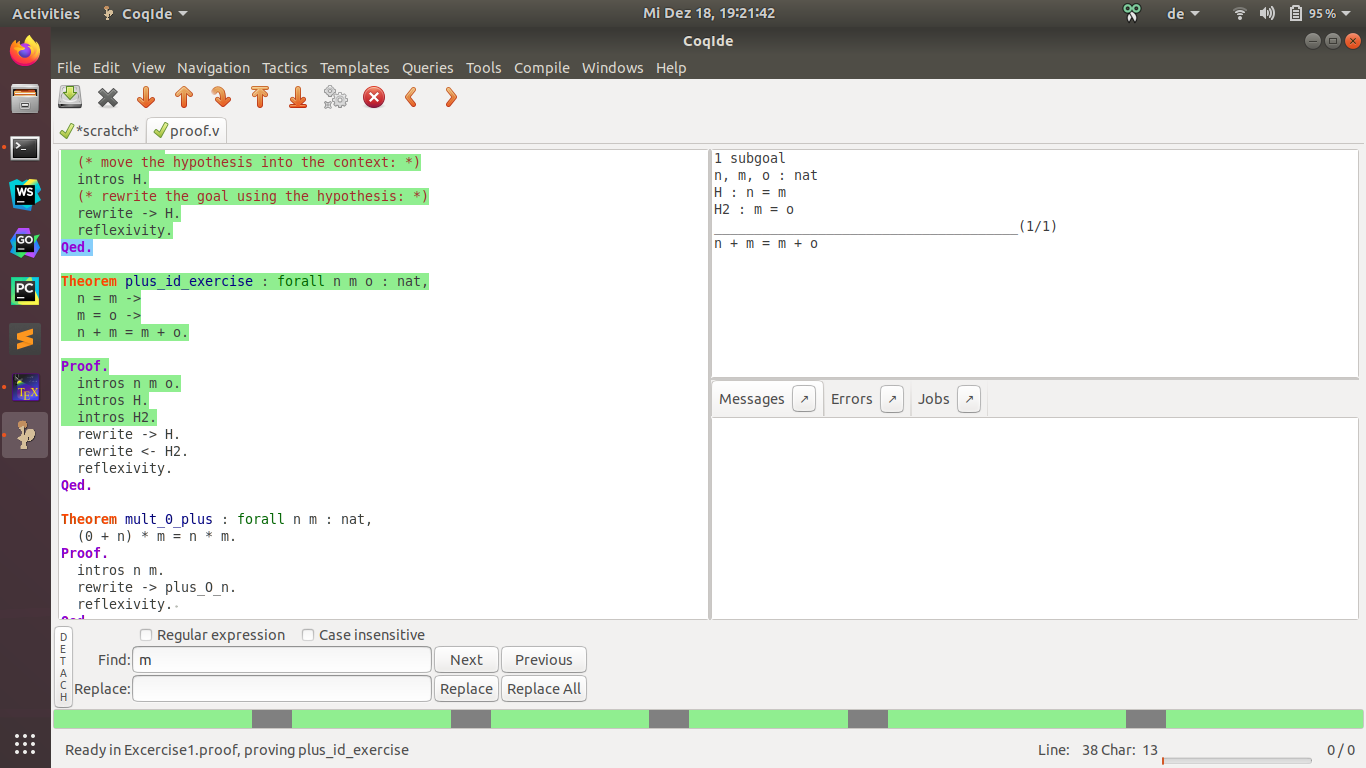
\includegraphics[width=1\textwidth]{\figdir/Coqide-sample.png}
	\caption{Coqide}
	\label{fig:coqide-sample}
\end{minipage}
Die Coqide bietet viele spezielle Features für formale Verifikation. Beispielsweise ist es möglich mit den Pfeilen in der Navigationsleiste die einzelnen Kommandos aus der linken Textbox auszuführen. Je nach Pfeil springt man einen Schritt vorwärts, bis zum Zeiger vorwärts oder auch rückwärts.\\
\\
Die Entwicklungsumgebung stellt grundsätzlich drei Fenster dar. Dabei wird eines für den Programmcode genutzt. Die anderen beiden Fenster auf der rechten Seite dienen ausschließlich der Informationsausgabe.\\
Im Screenshot ist ein Beweis zu sehen. Dabei wird überprüft, wenn die natürlichen Zahlen \textbf{n, m, o} und die Beziehungen \textbf{n = m} und \textbf{m = o} gegeben sind, dass \textbf{n + m = m + o} gilt.\\
Zunächst fällt auf, dass der Coq-Code teilweise grün markiert ist. Dies symbolisiert den bereits erfolgreich ausgeführten Teil. Das Ausgabefenster rechts oben zeigt, hierfür die passende Ausgabe. Dabei werden über dem Trennstrich die gegebenen Zahlen und Hypothesen angezeigt. Zusätzlich ist noch die Anzahl an Zielen abgebildet. Den darunter stehende Ausdruck gilt es zu beweisen.\\
Das dritte Fenster rechts unten dient zur Meldung von Hinweisen, Fehlern und Konsolenausgaben, wie beispielsweise von einer Suche.\\
\\
Im Anschluss folgt das bereits gezeigte Codebeispiel \ref{lst:sample-proof2} mit der ausführlichen Ausgabe der Coqide nach jedem Schritt.
Diese ist durch die Kommentarblöcke, welche durch \textbf{(*} eingeleitet und durch \textbf{*)} beendet werden, gekennzeichnet.
Wie bereits zuvor erklärt, gilt es, unter den gegebenen Umständen, \textbf{n + m = m + o} zu beweisen. Hierfür wird die \textbf{rewrite} Taktik eingesetzt. Nicht fachlich ausgedrückt bedeutet es, dass je nach Richtung des Pfeils die eine oder die andere Seite eingesetzt wird. Somit verändert sich die zu beweisende Aussage dynamisch im Coqide-Ausgabefeld. Nach dem ersten \textbf{Rewrite}, wird \textbf{n} mit \textbf{m} ersetzt. Das Einsetzen der zweiten Hypothese \textbf{H2} führt schlussendlich zu dem Ergebnis: \textbf{m + m = m + m}. Folglich kann das Ziel mit \textbf{reflexivity} bewiesen werden.
\begin{lstlisting}[language=coq,firstnumber=1,caption=Coq Beispielbeweis,label=lst:sample-proof2]
(* Initiating the theorem to proof. *)
Theorem plus_id_exercise : forall n m o : nat,
	n = m ->
	m = o ->
	n + m = m + o.
	
(* result: 
1 subgoal
______________________________________(1/1)
forall n m o : nat,
n = m -> m = o -> n + m = m + o*)

Proof.
(* move quantifiers into the context: *)
	intros n m o. 
	
(* result: 
1 subgoal
n, m, o : nat
______________________________________(1/1)
n = m -> m = o -> n + m = m + o*)

(* move hypothesises into the context: *)	
	intros H.
	intros H2.

(* result: 
1 subgoal
n, m, o : nat
H : n = m
H2 : m = o
______________________________________(1/1)
n + m = m + o*)

(* rewrite the goal using the hypothesises: *)
	rewrite -> H.

(* result: 
...
______________________________________(1/1)
m + m = m + o
*)
	rewrite <- H2.

(* result:
...
______________________________________(1/1)
m + m = m + m
*)
	reflexivity.
Qed.
\end{lstlisting}

\section{Coq und Programmcode}

Beim Zusammenspiel von Beweisen in Coq und Programmcode gibt es zwei verschiedene Richtungen. Einerseits können Theoreme bewiesen und dann in Programmiersprachen extrahiert werden. Andererseits ist es auch möglich, erst ein Programm zu entwickeln und anschließend dieses in Coq zu verifizieren. \\
Das dabei verwendete Prinzip lautet vereinfacht gesagt:
\textbf{Es gibt eine Liste von Dingen, die eine Software tun soll. Hierfür wird Logik verwendet, um zu beweisen, dass diese Software auch genau diese Dinge tut.}
\\
In den folgenden Unterkapiteln sind beide Wege beschrieben. Dabei wird die Richtung Proof zu Programm anhand eines genauen Codebeispiels erläutert.

\subsection{Proof -> Programm}
\subsubsection{theoretisch}
{Wie bereits zuvor erwähnt, ist der erste Schritt die Erstellung einer Spezifikation, welche die Software beschreibt. Anschließend muss diese in mathematischer Form in ein Proof Tool geschrieben und bewiesen werden. Auf fehlerhafte Beweise weißt dieses Tool hin.
Sobald jetzt ein Fehler in der realen Welt auftritt, sollte dieser mit diesem beschrieben Model abgefangen werden. \\
Schlussendlich müssen die bewiesenen Anforderungen der Spezifikation in Programmcode konvertiert werden. Dieser Prozess wird in folgendem Kapitel genauer erklärt.}\cite{HELWER01:FV}

\subsubsection{praktisch}
\begin{itemize}
	\item Programmcode in Coq bewiesen und dann in Ocaml extrahiert
	\item Ocaml ("`Categorical Abstract Machine + ML"') ist eine sowohl funktionale, als auch objektorientierte Programmiersprache.
	\item ML bedeutet Meta-Language. Dies ist für diese Arbeit weniger relevant, da Ocaml lediglich als Beispiel für Code-Extraction genutzt wird und der Fokus hauptsächlich auf dem Prinzip liegt.
	\item Code to Ocaml extractor ist nicht formal verifiziert. Korrektheit wird angenommen, da Coq in Ocaml geschrieben ist.
\end{itemize}
\textbf{Funktionalitäten schreiben und mathematisch beweisen}
\begin{itemize}
	\item natprod beschreibt ein paar von 2 natürlichen Zahlen
	\item Check und Compute wird als Konsolen-Ausgabe genutzt
	\item fst gibt x zurück
	\item snd gibt y zurück
	\item Notation ist ein Alias um bestimmte Ausdrücke anders als normal zu schreiben
	\item swap\_pair vertauscht x und y
	\item surjective\_pairing und surjective\_pairing\_stuck beweist, dass das Erstellen von einem neuem Paar demselben entspricht, wenn man fst und snd von diesem Paar nimmt und ein neues Paar bildet.
	\item snd\_fst\_is\_swap und fst\_swap\_is\_snd prüft die swap\_pair Funktion auf Korrektheit.
	\item destruct bedeutet: The tactic that tells Coq to consider, separately, the cases where n = O and where n = S n' is called destruct. The destruct generates two subgoals, which we must then prove, separately, in order to get Coq to accept the theorem. The same as we used in induction. The difference of destruct and induction is, that induction is capable of checking n = 0, n+1 and than say, if this is correct -> the whole proof is correct. In this example we use destruct just to split the pair p into n and m again. Otherwise Coq can't simplify the statement.
\end{itemize}

\begin{lstlisting}[language=coq,firstnumber=1,caption=Coq Beispielbeweis,label=lst:practical-proof]
From LF Require Export Induction.

Inductive natprod : Type :=
	| pair (n1 n2 : nat).

Check (pair 3 5).

Definition fst (p : natprod) : nat :=
match p with
	| pair x y => x
end.

Definition snd (p : natprod) : nat :=
match p with
	| pair x y => y
end.

Compute (fst (pair 3 5)).
Compute (snd (pair 5 7)).

Notation "( x , y )" := (pair x y).

Compute (fst (3,5)).
Definition fst' (p : natprod) : nat :=
match p with
	| (x,y) => x
end.
Definition snd' (p : natprod) : nat :=
match p with
	| (x,y) => y
end.
Definition swap_pair (p : natprod) : natprod :=
match p with
	| (x,y) => (y,x)
end.

Theorem surjective_pairing' : forall (n m : nat),
(n,m) = (fst (n,m), snd (n,m)).
Proof.
	simpl.
	reflexivity. 
Qed.

Theorem surjective_pairing_stuck : forall (p : natprod),
p = (fst p, snd p).
Proof.
	intros p.
	destruct p as [n m].  
	simpl.
	reflexivity.
Qed.

Theorem snd_fst_is_swap : forall(p : natprod),
(snd p, fst p) = swap_pair p.
Proof.
	intros p.
	destruct p as [n m].
	simpl.
	reflexivity.
Qed.

Theorem fst_swap_is_snd : forall(p : natprod),
fst (swap_pair p) = snd p.
Proof.
	intros p.
	destruct p as [n m].
	simpl.
	reflexivity.
Qed.
\end{lstlisting}
Um anschließend die formal bewiesenen Funktionen in Programmen nutzen zu können, muss die Datei, in der die Beweise geschrieben wurden, in Coq compiliert werden. Dafür muss folgender Befehl in die Kommandozeile eingeben werden:
\textbf{coqc -Q . LF PaperPair.v}. \\
\textbf{Coqc} ist hierbei der Aufruf des Coq-Compilers. \textbf{-Q . LF} sorgt dafür, dass alle .v-Dateien aus dem Paket LF in andere Coq-Dateien importiert werden können. Ein Paket in Coq ist ähnlich zu anderen Programmiersprachen wie beispielsweise Java.
\\
Für den nächsten Schritt in der Extraktion wird eine Coq-Datei benötigt, welche definiert, wie und was in welcher Sprache extrahiert werden soll. Diese muss ebenfalls über die Kommandozeile, wie zuvor beschrieben, compiliert werden.
\begin{lstlisting}[language=coq,firstnumber=1,caption=Coq Code extrahieren,label=lst:practical-proof-extraction]
Require Extraction.
Extraction Language OCaml.
Require Import ExtrOcamlBasic.
Require Import ExtrOcamlString.
Require Import Arith Even Div2 EqNat Euclid.

Extract Inductive nat => int [ "0" "Pervasives.succ" ]
"(fun fO fS n -> if n=0 then fO () else fS (n-1))".

Extraction "paperimpl.ml" fst snd swap_pair.
\end{lstlisting}
Im Codeblock \ref{lst:practical-proof-extraction} ist zu sehen, dass verschiedene Dateien mit \textbf{Require} und \textbf{Require Import} importiert werden. \textbf{Extraction} und \textbf{ExtraOcamlBasic} sind beispielweise Standard-Features von Coq um Funktionen von Coq-Code in Ocaml-Code umzuwandeln.\\
Weiterhin wird in der Zeile \textbf{Extract Inductive nat => \dots} ein Ausdruck verwendet, sodass OCaml den Typ der natürlichen Zahlen aus Coq verwenden kann.
Damit schlussendlich eine ausführbare Datei entsteht, muss definiert werden, welche Funktionen in welche Datei extrahiert werden sollen.\\
\\
Der folgende Code \ref{lst:practical-generated-code} ist das Resultat, des zuvor gezeigten Coq-Codes. 
\begin{lstlisting}[language=coq,firstnumber=1,caption=Ocaml Code anpassen,label=lst:practical-generated-code]
type natprod =
| Pair of int * int

(** val fst : natprod -> int **)

let fst = function
| Pair (x, _) -> x

(** val snd : natprod -> int **)

let snd = function
| Pair (_, y) -> y

(** val swap_pair : natprod -> natprod **)

let swap_pair = function
| Pair (x, y) -> Pair (y, x)
\end{lstlisting}
Dadurch das der Coq-To-Ocaml-Extraktor nicht komplett formal verifiziert ist, kann es sein, dass der Code nicht 100\% korrekt ist. Um sicherzustellen, dass dies der Fall ist, wurden im Nachhinein ein paar Tests geschrieben, welche im Codebeispiel \ref{lst:practical-code-adjustment} dargestellt werden. Diese Tests beschreiben einfache Funktionsaufrufe wie zum Beispiel das Erhalten des ersten und zweiten Wertes eines Paares. Anschließend werden die selben Funktionen noch einmal aufgerufen - allerdings auf ein neues Paar, dass du die swap\_	pair Funktion entstanden ist. Zur Nachvollziehbarkeit werden dabei die jeweiligen Ergebnisse auf der Kommandozeile ausgegeben.
\begin{lstlisting}[language=coq,firstnumber=1,caption=Ocaml Code anpassen,label=lst:practical-code-adjustment]
let pair = Pair(3, 4);;
let resultfst = fst pair;;
let resultsnd = snd pair;;

Printf.printf "Result fst: %d \n%!" resultfst;;
Printf.printf "Result snd: %d \n%!" resultsnd;;

let pair2 = swap_pair pair;;
let resultfst2 = fst pair2;;
let resultsnd2 = snd pair2;;

Printf.printf "Result fst: %d \n%!" resultfst2;;
Printf.printf "Result snd: %d \n%!" resultsnd2;;
\end{lstlisting}
Ocaml-Code muss genauso wie C-Code compiliert werden. Folgender Befehl ermöglicht es aus der \textbf{paperimpl.ml} und der \textbf{paperimpl.mli} Datei funktionierenden compilierten Code zu erhalten. Dieser wird unter dem Namen \textbf{paperimp} im selben Verzeichnis abgelegt.
\\
\begin{lstlisting}[language=coq,firstnumber=1,caption=Ocaml Code compilieren,label=lst:practical-code-compilation]
ocamlc -w -20 -w -26 -o paperimp paperimpl.mli paperimpl.ml
\end{lstlisting}

\begin{lstlisting}[language=coq,firstnumber=1,caption=Ocaml code ausführen,label=lst:practical-code-execution]
lukas@luk-ubuntu@~/Documents/coq-test/lf: ./paperimp
Result fst: 3 
Result snd: 4 
Result fst: 4 
Result snd: 3 
\end{lstlisting}
In Codeblock \ref{lst:practical-code-execution} werden die Ausgaben der Tests dargestellt. Die ersten zwei Ergebnisse sind die Werte, welches mit den Werten \textbf{fst: 3} und \textbf{snd: 4} initiiert wurde. Die zweiten zwei Ausgaben stellen \textbf{fst} und \textbf{snd} des invertierten Paars dar.

\subsection{Programm -> Proof}
\begin{itemize}
	\item nutze Verified Software Toolchain (VST) der PrincetonUniversity um C Code mathematisch zu beweisen
	\item Schreibe ein C Program F.c
	\item Führe clightgen -normalize F.c aus. Dadurch entsteht eine Datei Coq-File F.v
	\item Schreibe eine formale Verifikation in einer Datei (z.B.: verif\_F.v). In dieser File müssen sowohl F.v als auch das VST Floya Programm-Verifikationssystem VST.floyd.proofauto importieren.\cite{Appel01:VST}
\end{itemize}

\section{Aktuelle Anwendung}
\subsection{Proofed Stack}
\begin{itemize}
	\item CompCert (C compiler) \url{http://compcert.inria.fr}
	\item Princeton VST
	\item Certikos (verified Operating System with hypervisor and multi instances)
	\item \url{http://plv.csail.mit.edu/kami/}
	\item \url{https://www.zdnet.com/article/certikos-a-hacker-proof-os/}
	\item \url{https://github.com/PrincetonUniversity/VST}
	\item \url{https://vst.cs.princeton.edu}
	\item \url{https://news.yale.edu/2016/11/14/certikos-breakthrough-toward-hacker-resistant-operating-systems}
\end{itemize}
\subsection{JSCert for ECMA 5}
\url{https://github.com/jscert/jscert}
\subsection{4-Farben Rätsel ist löstbar!}
\url{http://www.ams.org/notices/200811/tx081101382p.pdf}
\subsection{CertiCoq}
\url{https://www.cs.princeton.edu/~appel/papers/certicoq-coqpl.pdf}

\section{Aufwand in der Praxis}
\begin{itemize}
	\item Für jede Zeile Code wurden >= 5 extra Zeilen Proofs geschrieben.
	\item Code der geschrieben wurde, hat meistens sofort funktioniert. (Es ist eine neue Art zu programmieren)
	\item Projekt Ironclad von Microsoft Research. Talk von Bryan Parno 2014 \url{https://www.usenix.org/node/186162}
	\item Objektorientierung eher schwer, da direkte Umwandlung von funktionaler Sprache in eine funktionale Sprache einfacher ist. (Außerdem programmieren die Menschen, die das entwickeln eigentlich nicht wirklich objektorientiert)
\end{itemize}


\section{Fazit}
\begin{itemize}
	\item Programmcodeverifikation nimmt vor allem in sicherheitskritischen Bereichen zu
	\item Programmcodeverifikation ist deutlich zeitintensiver (5mal)
	\item Mit dieser Verifikation kann 100\%tige Garantie für funktionierende Software gewährleistet werden
	\item Es hat großes Potential
	\item Wird sehr stark durch die Community weiterentwickelt
	\item Große Firmen nutzen es immer aktiver
	\item nur Software kann sicher gemacht werden. Hardware ist immer noch fehlbar!
\end{itemize}

\section{Glossar}


%%% Local Variables: 
%%% mode: latex
%%% TeX-master: "thesis.tex"
%%% End: 
